\chapter{Quadratic functions}
\section{Defined on $\mdr$}
Let $f(x) = a \cdot x^2 + b \cdot x + c$ with $a \in \mdr \setminus \Set{0}$ and 
$b, c \in \mdr$ be a quadratic function.

\begin{figure}[htp]
    \centering
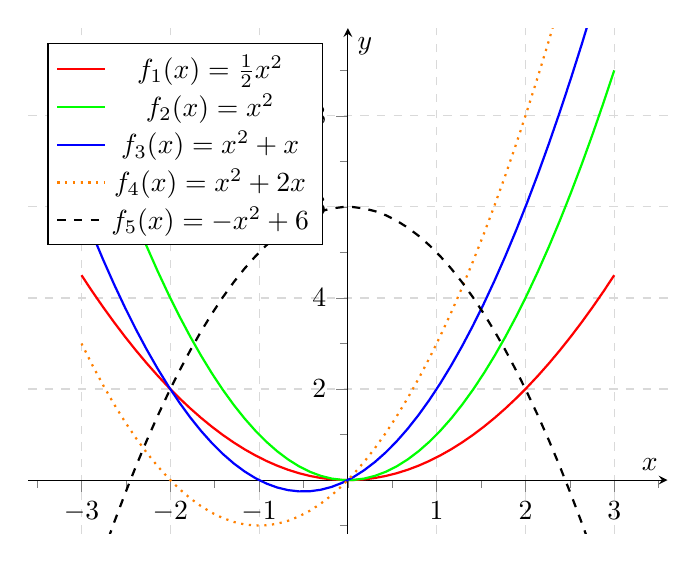
\begin{tikzpicture}
    \begin{axis}[
        legend pos=north west,
        axis x line=middle,
        axis y line=middle,
        grid = major,
        width=0.8\linewidth,
        height=8cm,
        grid style={dashed, gray!30},
        xmin=-3,    % start the diagram at this x-coordinate
        xmax= 3,    % end   the diagram at this x-coordinate
        ymin=-0.25, % start the diagram at this y-coordinate
        ymax= 9,    % end   the diagram at this y-coordinate
        axis background/.style={fill=white},
        xlabel=$x$,
        ylabel=$y$,
        tick align=outside,
        minor tick num=-3,
        enlargelimits=true,
        tension=0.08]
      \addplot[domain=-3:3, thick,samples=50, red]    {0.5*x*x}; 
      \addplot[domain=-3:3, thick,samples=50, green]  { x*x}; 
      \addplot[domain=-3:3, thick,samples=50, blue]   { x*x +   x};
      \addplot[domain=-3:3, thick,samples=50, orange,dotted] { x*x + 2*x};
      \addplot[domain=-3:3, thick,samples=50, black,dashed]  {-x*x + 6};
      \addlegendentry{$f_1(x)=\frac{1}{2}x^2$}
      \addlegendentry{$f_2(x)=x^2$}
      \addlegendentry{$f_3(x)=x^2+x$}
      \addlegendentry{$f_4(x)=x^2+2x$}
      \addlegendentry{$f_5(x)=-x^2+6$}
    \end{axis} 
\end{tikzpicture}
    \caption{Quadratic functions}
\end{figure}

\subsection{Calculate points with minimal distance}
In this case, $d_{P,f}^2$ is polynomial of degree 4. 
We use Theorem~\ref{thm:required-extremum-property}:\nobreak
\begin{align}
    0     &\overset{!}{=} (d_{P,f}^2)'\\
          &= -2 x_p + 2x -2y_p f'(x) + \left (f(x)^2 \right )'\\
          &= -2 x_p + 2x -2y_p f'(x) + 2 f(x) \cdot f'(x) \rlap{\hspace*{3em}(chain rule)}\label{eq:minimizingFirstDerivative}\\
\Leftrightarrow 0 &\overset{!}{=} -x_p + x -y_p f'(x) + f(x) \cdot f'(x) \rlap{\hspace*{3em}(divide by 2)}\label{eq:minimizingFirstDerivative}\\
          &= -x_p + x -y_p (2ax+b) + (ax^2+bx+c)(2ax+b)\\
          &= -x_p + x -y_p \cdot 2ax- y_p b + (2 a^2 x^3+2 a b x^2+2 a c x+ab x^2+b^2 x+bc)\\
          &= -x_p + x -2y_p ax- y_p b + (2a^2 x^3 + 3 ab x^2 + 2acx + b^2 x + bc)\\
          &= 2a^2 x^3 + 3 ab x^2 + (1 -2y_p a+ 2ac + b^2)x +(bc-by_p-x_p)\label{eq:quadratic-derivative-eq-0}
\end{align}

This is an algebraic equation of degree 3.
There can be up to 3 solutions in such an equation. Those solutions
can be found with a closed formula.

\todo[inline]{Where are those closed formulas?}

\begin{example}
    Let $a = 1,  b = 0,  c= 1, x_p= 0, y_p = 1$.
    So $f(x) = x^2 + 1$ and $P(0, 1)$.

\begin{align}
    0 &\stackrel{!}{=} 4 x^3 - 2x\\
      &=2x(2x^2 - 1)\\
    \Rightarrow x_1 &= 0 \;\;\; x_{2,3} = \pm \frac{1}{\sqrt{2}}
\end{align}

As you can easily verify, only $x_1$ is a minimum of $d_{P,f}$.
\end{example}


\subsection{Number of points with minimal distance}
\begin{theorem}
    A point $P$ has either one or two points on the graph of a 
    quadratic function $f$ that are closest to $P$.
\end{theorem}

In the following, I will do some transformations with $f = f_0$ and
$P = P_0$ .

Moving $f_0$ and $P_0$ simultaneously in $x$ or $y$ direction does 
not change the minimum distance. Furthermore, we can find the 
points with minimum distance on the moved situation and calculate
the minimum points in the original situation.

First of all, we move $f_0$ and $P_0$ by $\frac{b}{2a}$ in $x$ direction, so
\[f_1(x) = ax^2 - \frac{b^2}{4a} + c \;\;\;\text{ and }\;\;\; P_1 = \left (x_p+\frac{b}{2a},\;\; y_p \right )\]

Because:\footnote{The idea why you subtract $\frac{b}{2a}$ within
$f$ is that when you subtract something from $x$ before applying
$f$ it takes more time ($x$ needs to be bigger) to get to the same
situation. So to move the whole graph by $1$ to the left whe have
to add $+1$.}
\begin{align}
    f(x-\nicefrac{b}{2a}) &= a (x-\nicefrac{b}{2a})^2 + b (x-\nicefrac{b}{2a}) + c\\
    &= a (x^2 - \nicefrac{b}{a} x + \nicefrac{b^2}{4a^2}) + bx - \nicefrac{b^2}{2a} + c\\
    &= ax^2 - bx + \nicefrac{b^2}{4a} + bx - \nicefrac{b^2}{2a} + c\\
    &= ax^2 -\nicefrac{b^2}{4a} + c
\end{align}


Then move $f_1$ and $P_1$ by $\frac{b^2}{4a}-c$ in $y$ direction. You get:
\[f_2(x) = ax^2\;\;\;\text{ and }\;\;\; P_2 = \Big (\underbrace{x_P+\frac{b}{2a}}_{=: z},\;\; \underbrace{y_P+\frac{b^2}{4a}-c}_{=: w} \Big )\]

\textbf{Case 1:} As $f_2(x) = ax^2$ is symmetric to the $y$ axis, only points 
$P = (0, w)$ could possilby have three minima.

Then compute:
\begin{align}
  d_{P,{f_2}}(x)  &= \sqrt{(x-0)^2 + (f_2(x)-w)^2}\\
    &= \sqrt{x^2 + (ax^2-w)^2}\\
    &= \sqrt{x^2 + a^2 x^4-2aw x^2+w^2}\\
    &= \sqrt{a^2 x^4 + (1-2aw) x^2 + w^2}\\
    &= \sqrt{\left (a^2 x^2 + \frac{1-2 a w}{2} \right )^2 + w^2 - (1-2 a w)^2}\\
    &= \sqrt{\left (a^2 x^2 + \nicefrac{1}{2}-a w \right )^2 + \big (w^2 - (1-2 a w)^2 \big)}
\end{align}

The term 
\[a^2 x^2 + (\nicefrac{1}{2}-a w)\]
should get as close to $0$ as possilbe when we want to minimize 
$d_{P,{f_2}}$. For $w \leq \nicefrac{1}{2a}$ you only have $x = 0$ as a minimum.
For all other points $P = (0, w)$, there are exactly two minima $x_{1,2} = \pm \sqrt{aw - \nicefrac{1}{2}}$.

\textbf{Case 2:} $P = (z, w)$ is not on the symmetry axis, so $z \neq 0$. Then you compute:
\begin{align}
  d_{P,{f_2}}(x)  &= \sqrt{(x-z)^2 + (f(x)-w)^2}\\
    &= \sqrt{(x^2 - 2zx + z^2) + ((ax^2)^2 - 2 awx^2 + w^2)}\\
    &= \sqrt{a^2x^4 + (1- 2 aw)x^2 +(- 2z)x + z^2 + w^2}\\
  0 &\stackrel{!}{=} \Big(\big(d_{P, {f_2}}(x)\big)^2\Big)' \\
    &= 4a^2x^3 + 2(1- 2 aw)x +(- 2z)\\
    &= 2 \left (2a^2x^2 + (1- 2 aw) \right )x - 2z\\
    \Leftrightarrow 0 &\stackrel{!}{=} (2a^2x^2  + (1- 2 aw)) x - z\\
    &= 2 a^2 x^3 + (1- 2 aw) x - z\\
\Leftrightarrow 0 &\stackrel{!}{=} x^3 + \underbrace{\frac{(1- 2 aw)}{2 a^2}}_{=: \alpha} x  + \underbrace{\frac{-z}{2 a^2}}_{=: \beta}\\
    &= x^3 + \alpha x + \beta\label{eq:simple-cubic-equation-for-quadratic-distance}
\end{align}

The solution of Equation~\ref{eq:simple-cubic-equation-for-quadratic-distance}
is
\[t := \sqrt[3]{\sqrt{3 \cdot (4 \alpha^3 + 27 \beta^2)} -9\beta}\]
\[x = \frac{t}{\sqrt[3]{18}} - \frac{\sqrt[3]{\frac{2}{3}} \alpha }{t}\]

When you insert this in Equation~\ref{eq:simple-cubic-equation-for-quadratic-distance}
you get:\footnote{Remember: $(a-b)^3 = a^3-3 a^2 b+3 a b^2-b^3$}
\allowdisplaybreaks
\begin{align}
    0 &\stackrel{!}{=} \left (\frac{t}{\sqrt[3]{18}} - \frac{\sqrt[3]{\frac{2}{3}} \alpha }{t} \right )^3 + \alpha \left (\frac{t}{\sqrt[3]{18}} - \frac{\sqrt[3]{\frac{2}{3}} \alpha }{t} \right ) + \beta\\
&= (\frac{t}{\sqrt[3]{18}})^3 
    - 3 (\frac{t}{\sqrt[3]{18}})^2 \frac{\sqrt[3]{\frac{2}{3}} \alpha }{t} 
    + 3 (\frac{t}{\sqrt[3]{18}})(\frac{\sqrt[3]{\frac{2}{3}} \alpha }{t})^2 
    - (\frac{\sqrt[3]{\frac{2}{3}} \alpha }{t})^3 
    + \alpha \left (\frac{t}{\sqrt[3]{18}} - \frac{\sqrt[3]{\frac{2}{3}} \alpha }{t} \right ) + \beta\\
&= \frac{t^3}{18}             
    - \frac{3t^2}{\sqrt[3]{18^2}} \frac{\sqrt[3]{\frac{2}{3}} \alpha }{t}
    + \frac{3t}{\sqrt[3]{18}} \frac{\sqrt[3]{\frac{4}{9}} \alpha^2 }{t^2} 
    - \frac{\frac{2}{3} \alpha^3 }{t^3} 
    + \alpha \left (\frac{t}{\sqrt[3]{18}} - \frac{\sqrt[3]{\frac{2}{3}} \alpha }{t} \right ) + \beta\\
&= \frac{t^3}{18}
    - \frac{\sqrt[3]{18} t \alpha}{\sqrt[3]{18^2}}
    + \frac{\sqrt[3]{12} \alpha^2}{\sqrt[3]{18} t}  
    - \frac{\frac{2}{3} \alpha^3 }{t^3} 
    + \alpha \left (\frac{t}{\sqrt[3]{18}} - \frac{\sqrt[3]{\frac{2}{3}} \alpha }{t} \right ) + \beta\\
&= \frac{t^3}{18} 
    - \frac{t \alpha}{\sqrt[3]{18}} 
    \color{red}+ \frac{\sqrt[3]{2} \alpha^2}{\sqrt[3]{3} t} \color{black}
    - \frac{\frac{2}{3} \alpha^3 }{t^3} 
    + \color{red}\alpha \color{black} \left (\frac{t}{\sqrt[3]{18}}  \color{red}- \frac{\sqrt[3]{\frac{2}{3}} \alpha }{t} \color{black}\right ) 
    + \beta\\
&= \frac{t^3}{18} \color{blue}- \frac{t \alpha}{\sqrt[3]{18}} \color{black} 
    - \frac{\frac{2}{3} \alpha^3 }{t^3} 
    \color{blue}+ \frac{\alpha t}{\sqrt[3]{18}} \color{black} 
    + \beta\\
&= \frac{t^3}{18} - \frac{\frac{2}{3} \alpha^3 }{t^3} + \beta\\
&= \frac{t^6 - 12 \alpha^3 + \beta 18 t^3}{18t^3}
\end{align}

Now only go on calculating with the numerator. Start with resubstituting
$t$:
\begin{align}
0 &= (\sqrt{3 \cdot (4 \alpha^3 + 27 \beta^2)} -9\beta)^2 - 12 \alpha^3 + \beta 18 (\sqrt{3 \cdot (4 \alpha^3 + 27 \beta^2)} -9\beta)\\
&= (\sqrt{3 \cdot (4 \alpha^3 + 27 \beta^2)})^2 +(9\beta)^2 - 12 \alpha^3 -18\cdot 9\beta^2\\
&= 3 \cdot (4 \alpha^3 + 27 \beta^2) -81 \beta^2 - 12 \alpha^3\\
&= (4 \alpha^3 + 27 \beta^2) -27 \beta^2 - 4 \alpha^3\\
&= 0
\end{align}

\goodbreak
So the solution is given by
\begin{align*}
x_S &:= - \frac{b}{2a} \;\;\;\;\; \text{(the symmetry axis)}\\
w &:= y_P+\frac{b^2}{4a}-c \;\;\; \text{ and } \;\;\; z := x_P+\frac{b}{2a}\\
\alpha &:= \frac{(1- 2 aw)}{2 a^2} \;\;\;\text{ and }\;\;\; \beta := \frac{-z}{2 a^2}\\
t &:= \sqrt[3]{\sqrt{3 \cdot (4 \alpha^3 + 27 \beta^2)} -9\beta}\\
\underset{x\in\mdr}{\arg \min d_{P,f}(x)} &= \begin{cases}
     x_1 = +\sqrt{a (y_p + \frac{b^2}{4a} - c) - \frac{1}{2}} + x_S \text{ and }   &\text{if } x_P = x_S \text{ and } y_p + \frac{b^2}{4a} - c >  \frac{1}{2a} \\
     x_2 = -\sqrt{a (y_p + \frac{b^2}{4a} - c) - \frac{1}{2}} + x_S\\
     x_1 = x_S   &\text{if } x_P = x_S \text{ and } y_p + \frac{b^2}{4a} - c \leq  \frac{1}{2a} \\
     x_1 = \frac{t}{\sqrt[3]{18}} - \frac{\sqrt[3]{\frac{2}{3}} \alpha }{t}   &\text{if } x_P \neq x_S
    \end{cases}
\end{align*}

\section{Defined on a closed interval of $\mdr$}
